% Created 2021-01-24 Sun 22:49
% Intended LaTeX compiler: pdflatex
\documentclass[11pt]{article}
\usepackage[utf8]{inputenc}
\usepackage[T1]{fontenc}
\usepackage{graphicx}
\usepackage{grffile}
\usepackage{longtable}
\usepackage{wrapfig}
\usepackage{rotating}
\usepackage[normalem]{ulem}
\usepackage{amsmath}
\usepackage{textcomp}
\usepackage{amssymb}
\usepackage{capt-of}
\usepackage{hyperref}
\usepackage{minted}
\hypersetup{colorlinks=true, linkcolor=black, filecolor=red, urlcolor=blue}
\usepackage[turkish]{babel}
\author{Eren Hatırnaz}
\date{9 Şubat 2020}
\title{Yazılım Gündemi - 2020/06\\\medskip
\large 3-9 Şubat 2020}
\hypersetup{
 pdfauthor={Eren Hatırnaz},
 pdftitle={Yazılım Gündemi - 2020/06},
 pdfkeywords={},
 pdfsubject={},
 pdfcreator={Emacs 27.1 (Org mode 9.3)},
 pdflang={Turkish}}
\begin{document}

\maketitle
\tableofcontents \clearpage\shorthandoff{=}

\begin{center}
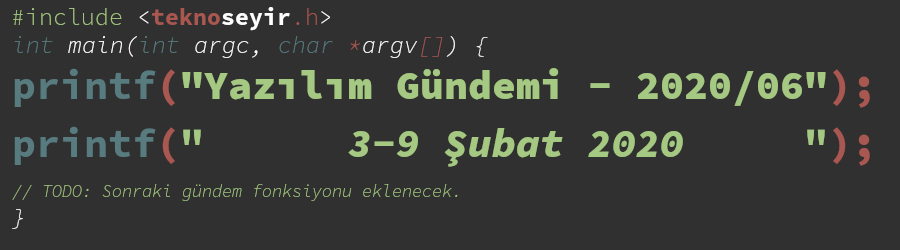
\includegraphics[width=.9\linewidth]{gorseller/yazilim-gundemi-banner.png}
\end{center}

\begin{center}
\href{../05/yazilim-gundemi-2020-05.pdf}{< Önceki Gündem} | \textbf{3-9 Şubat 2020} | \href{../07/yazilim-gundemi-2020-07.pdf}{Sonraki Gündem >}

\href{https://teknoseyir.com/blog/yazilim-gundemi-2020-06}{TeknoSeyir'de Oku}
\end{center}

\section{Google Chrome tarayıcısının SameSite Cookie değişiklikleri \href{https://blog.chromium.org/2020/02/samesite-cookie-changes-in-february.html}{bu ay devreye giriyor}}
\label{sec:org530a45e}
Bir fikr-i takip haberi yapalım. Bu konudan \href{../../2019/15/yazilim-gundemi-15.pdf}{Yazılım Gündemi - 15} yazısında
bahsetmiştik. Bu nedenle değişiklikle ilgili detaylı bilgi edinmek isterseniz
o yazıya bakabilirsiniz ama şöyle kısa bir bilgi de verelim. 4 Şubat tarihinde
yayınlanan Chrome 80 sürümü ile hayatımıza giren SameSite Cookie özelliği,
sitelerde bulunan üçüncü parti çerezlerin \texttt{SameSite=None;Secure} ifadesi ile
işaretlenmesi gerekliliğini getiriyor. Bu özellik sayesinde çerezler güvenli
bağlantılar arasında işlenebilecek. Tarayıcınızın bu özelliği destekleyip
desteklemediğine \href{https://samesite-sandbox.glitch.me/}{bu sayfadan} bakabilirsiniz. Sayfadaki her şeyin yeşil olması
gerekiyor.

Eğer sitenizde bir çerez üçüncü parti olduğu halde yukarıdaki gibi
işaretlenmemişse Chrome 80 sürümünün Geliştirici Araçları konsol ekranında
aşağıdaki gibi bir uyarı ile karşılaşacaksınız.

\begin{center}
\includegraphics[width=.9\linewidth]{gorseller/chrome-samesite-developer-tools-uyarı.png}
\end{center}

Bu durumda sizin yapacağınız pek bir şey yok gibi gözüküyor, sayfanıza
eklediğiniz servisin ilgili değişiklikleri yapmasını bekleyeceksiniz ama eğer
siz böyle bir servis sunuyorsanız o zaman \href{https://web.dev/samesite-cookies-explained/}{şu yazıyı} okumanızda fayda var.
Fakat bazı servisler geriye uyumluluk olması açısından aynı çerezden iki tane
kullanabilir, yani birisi eski, diğeri yeni ayarlarda iki çerez yukarıdaki
uyarı bunlardan birisi için de gözükebilir, nitekim Google'ın bazı
servislerinde de durum böyle olabilecekmiş.

\begin{itemize}
\item \href{https://www.youtube.com/watch?v=GPz7onXjP\_4}{Konuyla ilgili YouTube videosu}
\end{itemize}

Daha detaylı bilgi ve ileri okuma kaynakları için konu başlığına eklediğim
bağlantıyı inceleyebilirsiniz.
\section{\href{https://snyk.io/blog/jvm-ecosystem-report-2020/}{JVM Ekosistem Raporu 2020} yayınlandı.}
\label{sec:org6406743}
\begin{figure}[htbp]
\centering
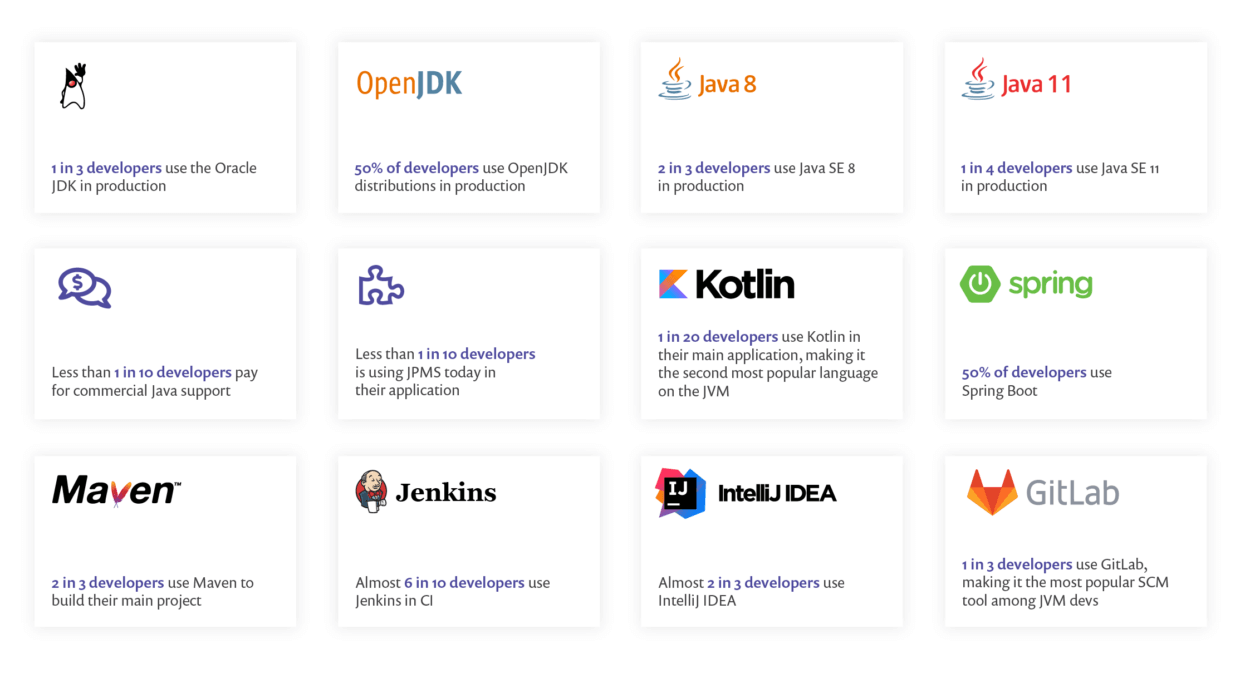
\includegraphics[width=.9\linewidth]{gorseller/jvm-ekosistem-2020-ozet.png}
\caption{Anket sonuçlarının özeti}
\end{figure}

Snyk isimli firmanın düzenlemiş olduğu JVM (Java Virtual Machine) ekosistemi
anketinin sonuçları bu hafta içerisinde yayınlandı. Yukarıdaki görselde
gördüğünüz özetin tam halini incelemek için \href{https://snyk.io/wp-content/uploads/jvm\_2020.pdf}{bu adresteki PDF dosyası}nı
inceleyebilirsiniz.

\begin{figure}[htbp]
\centering
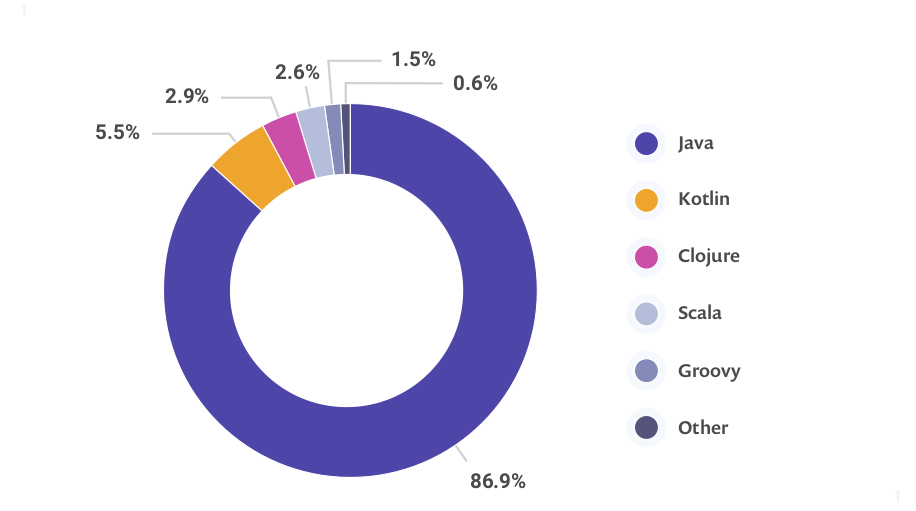
\includegraphics[width=.9\linewidth]{gorseller/jvm-ekosistem-2020-diller.png}
\caption{JVM üzerinde çalışan diller arasında Kotlin yükselişte.}
\end{figure}
\newpage
\section{TypeScript 3.8 RC \href{https://devblogs.microsoft.com/typescript/announcing-typescript-3-8-rc/}{sürümü yayınlandı}}
\label{sec:orgda5b38d}
Geçtiğimiz haftalardaki yazılım gündemi yazısında (bkz: \href{../02/yazilim-gundemi-2020.02.pdf}{Yazılım Gündemi -
2020/02}) Beta sürümünün yayınlandığını duyurduğum TypeScript dilinin bu hafta
Relase Candidate sürümü yayınlandı. Bu sürümle birlikte gelen "Private Fields"
özelliğine o yazına değinmiştim. Diğer özellikleri de inceledim fakat aktif
olarak kullandığım bir dil olmadığı için pek bir şey anladığımı
söyleyemeyeceğim. Bu nedenle ilgili arkadaşları konu başlığına eklediğim
bağlantıyı okumaya davet etmekten başka yapabileceğim bir şey yok. Bir sonraki
sürümde dersime çalışmayı deneyeceğim :)
\section{Angular 9 \href{https://blog.angular.io/version-9-of-angular-now-available-project-ivy-has-arrived-23c97b63cfa3}{sürümü yayınlandı}}
\label{sec:org8482ff0}
VueJS ve ReactJS gibi kütüphanelerin çıkmasıyla birlikte her ne kadar
popülerliği azalmış olsa da kurumsal camiada hala daha kullanılmaya devam
edilen Angular kütüphanesinin bu hafta içerisinde 9.0.0 sürümü yayınlandı.
Front-End tarafına çok uzak biri sayılmam aslında ama bir projede Angular
kullanmayalı bayağı uzun zaman oluyor o yüzden pek fazla detaylara
inemeyeceğim.

Bu sürüm, \href{https://angular.io/guide/ivy}{Ivy} ismini verdikleri derleme ve çalışma zamanında render yapma
kısımlarında çalışan bir "derleyici" ile birlikte geliyor ve Angular takımının
iddiasına göre şunları sunuyormuş:

\begin{itemize}
\item Daha küçük paket boyutları.
\item Daha hızlı test.
\item Daha iyi debugging.
\item CSS class ve style tanımlamaları iyileştirilmiş.
\item Tip kontrolü iyileştirilmiş.
\item Derleme hataları ve derleme zamanı iyileştirilmiş.
\item Çoklu dil desteği iyileştirilmiş.
\end{itemize}

\begin{figure}[htbp]
\centering
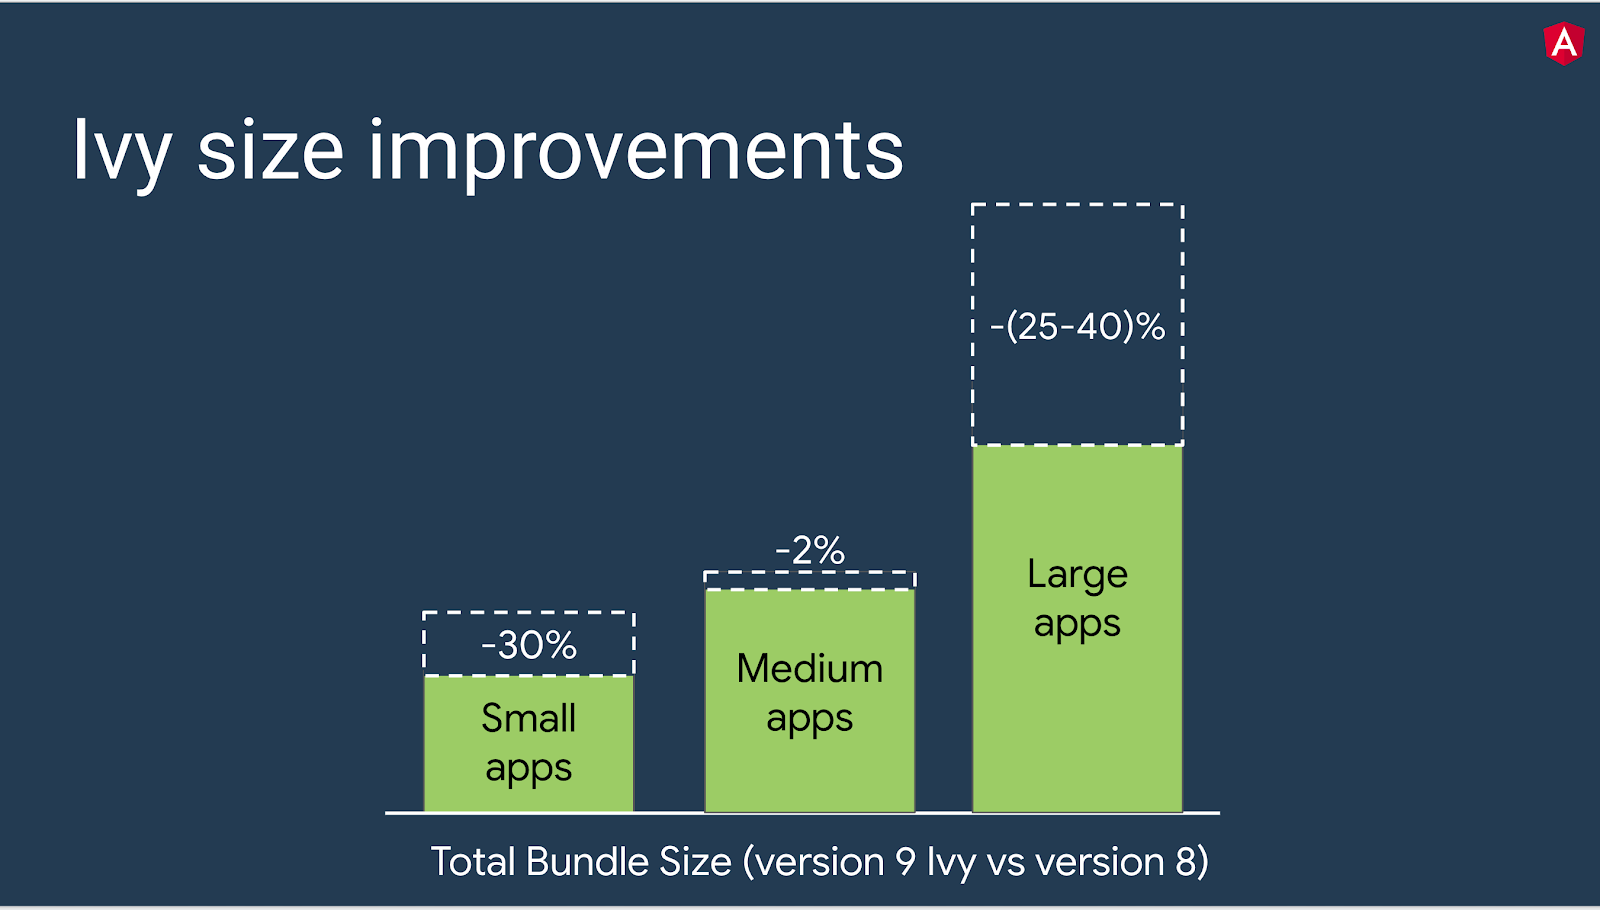
\includegraphics[width=.9\linewidth]{gorseller/angular9-paket-boyutlari.png}
\caption{Uygulama boyutlarına göre Angular 9'un küçülme oranları.}
\end{figure}

Yukarıdaki grafikte görebileceğiniz üzere Ivy isimli "derleyici" ile birlikte
uygulamanızın boyutlarına göre dikkate değer bir paket boyutu azalması söz
konusu. Bu da demek oluyor ki artık uygulamalarınız hem daha az yer
kaplayacak, hem de kullanılmayan gereksiz komponentler atıldığı için daha
hızlı yüklenme sürelerine sahip olacaksınız. Angular'ın genelde çok büyük
paket boyutundan dolayı pek fazla tercih edilmediği düşünüldüğünde bu gelişme
iyi bir adım diyebiliriz ama VueJS ve ReactJS kullananları kendine çekebilir
mi bilinmez.

Bu sürüme yükseltmek için aşağıdaki komutları kullanabilirsiniz ama öncesinde
şu sayfadaki Angular Güncelleme Rehberi'ni okumanızı şiddetle tavsiye ederim:
\url{https://update.angular.io/}

\begin{verbatim}
$ ng update @angular/cli @angular/core
\end{verbatim}
\section{Swift 5.2 \href{https://www.hackingwithswift.com/articles/212/whats-new-in-swift-5-2}{sürümü yayınlandı}}
\label{sec:org45b4e22}
Apple tarafından geliştirilen ve çoğunlukla yine Apple ekosistemindeki
cihazlar için uygulama geliştirmek için kullanılan programlama dili Swift'in
5.2 sürümü bu hafta içerisinde yayınlandı. Mobil uygulama geliştirme tarafına
çok uzak birisi olsam da blog yazılarındaki kodları ve yapıları kolayca
anlayabildim. O halde gelin bir özelliği birlikte inceleyelim:
\subsection{Key Path Expressions as Functions (\href{https://github.com/apple/swift-evolution/blob/master/proposals/0249-key-path-literal-function-expressions.md}{SE-0249})}
\label{sec:orgee9a48e}
Hemen her programlama dilinde bulunan, dizi içerisinde çeşitli işlemler
yapılabilen \texttt{map}, \texttt{filter} gibi fonksiyonlar Swift dilinde de var fakat
bu sürümde bir kolaylık geldi. Örnek üzerinden anlatmak gerekirse:

Diyelim bu şekilde bir struct tanımınız var:
\begin{minted}[breaklines=true,breakanywhere=true,frame=lines, linenos, label=Swift, labelposition=topline]{swift}
struct Kullanici {
    let isim: String
    let yas: Int

    var oyKullanabilirMi: Bool {
        yas >= 18
    }
}
\end{minted}

ve bu şekilde objelerimiz olsun:
\begin{minted}[breaklines=true,breakanywhere=true,frame=lines, linenos, label=Swift, labelposition=topline]{swift}
let eren = Kullanici(isim: "Eren Hatırnaz", yas: 25)
let ahmet = Kullanici(isim: "Ahmet Mehmetoğlu", yas: 17)
let mehmet = Kullanici(isim: "Mehmet Ahmetoğlu", yas: 18)

let kullanicilar =  [eren, ahmet, mehmet]
\end{minted}

ve bu \texttt{kullanicilar} dizisindeki elemanların isimlerini getirmemiz gerekir.
Eskiden bu şekilde yapıyorduk:
\begin{minted}[breaklines=true,breakanywhere=true,frame=lines, linenos, label=Swift, labelposition=topline]{swift}
let eski_kullaniciAdlari = kullanicilar.map { $0.isim }
\end{minted}
Artık bu şekilde kullanabiliyoruz:
\begin{minted}[breaklines=true,breakanywhere=true,frame=lines, linenos, label=Swift, labelposition=topline]{swift}
let kullaniciAdlari = kullanicilar.map(\.isim)
print(kullaniciAdlari)
\end{minted}
Aynı şekilde \texttt{filter} ve diğer fonksiyonlar için de bu şekilde kullanmak
mümkün:
\begin{minted}[breaklines=true,breakanywhere=true,frame=lines, linenos, label=Swift, labelposition=topline]{swift}
let oyKullanabilenler = kullanicilar.filter(\.oyKullanabilirMi)
\end{minted}

Bu arada ilk defa gördüğüm için söylemeden edemeyeceğim. Swift'in söz dizimi
gerçekten güzelmiş. Özellike bu \texttt{oyKullanabilirMi} özelliğini tanımlarken
kullandığım \texttt{yas} değeri 18'den büyükse \texttt{True} olsun anlamına gelen söz dizimi
gerçekten çok zekice.

Bu sürüm ile birlikte dile başka birçok özellik daha eklendi fakat hepsine
değinirsem yazı çok uzayacak. Bu nedenle ilgili arkadaşları konu başlığına
eklediğim bağlantıya tıklamaya davet ediyorum.

Ayrıca bu hafta başında Swift takımı Swift Crypto isimli yeni bir \href{https://swift.org/blog/crypto/}{açık kaynak
proje de duyurdu}. \href{https://github.com/apple/swift-crypto}{GitHub deposu}
\section{GNU ve Özgür Yazılım Vakfı (FSF) \href{https://www.gnu.org/gnu/2020-announcement-1.html}{birlikte çalışmaya devam edecek}}
\label{sec:org6961702}
Richard Stallman'ın olayından (bkz: \href{../../2019/10/yazilim-gundemi-10.pdf}{Yazılım Gündemi - 10}) sonra GNU oluşumu
ile Free Software Foundation arasındaki ilişkiler de tartışmalı duruma
gelmişti (bkz: \href{../../2019/13/yazilim-gundemi-13.pdf}{Yazılım Gündemi - 13}). Bu hafta iki tarafında kendi sitelerine
ekledikleri sayfadaki (\href{https://www.gnu.org/gnu/2020-announcement-1.html}{GNU}, \href{https://www.fsf.org/news/gnu-fsf-cooperation-update}{FSF}) yazı ile birlikte bu olaylar biraz çözülmüş
gibi gözüküyor. Her ne kadar iletişimlerini minimum seviyeye indirmek
istediklerini belirtseler de birlikte çalışmaya devam edeceklermiş. Yine de
konuyla ilgili fikir belirtmek isteyenlerin 13 Şubat tarihine kadar süresi
varmış.
\section{Visual Studio v1.42 (Ocak 2020) \href{https://code.visualstudio.com/updates/v1\_42}{sürümü yayınlandı}}
\label{sec:orgdf54201}
\begin{center}
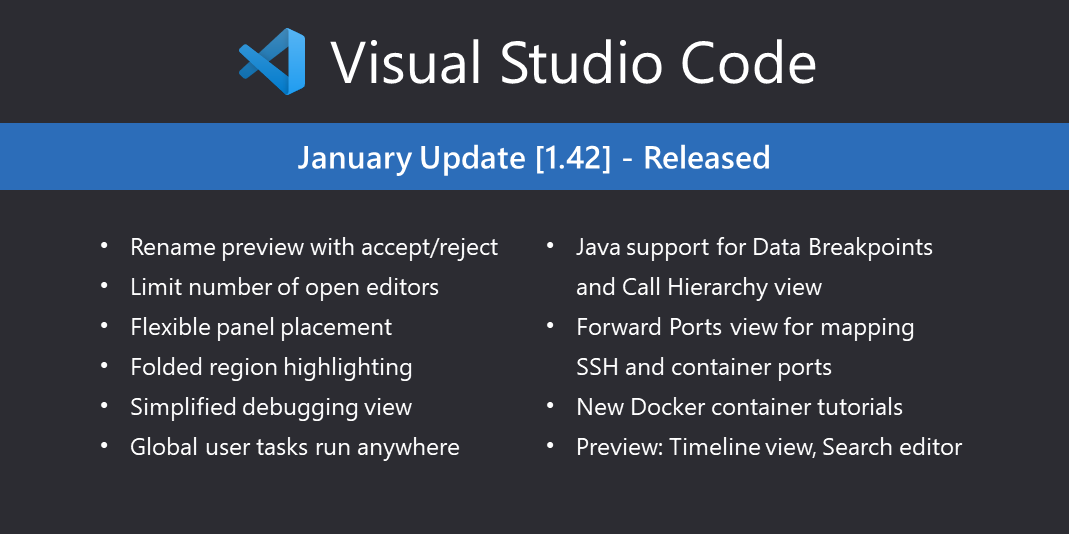
\includegraphics[width=.9\linewidth]{gorseller/vscode-142.png}
\end{center}
\section{Yaklaşan Etkinlikler}
\label{sec:org30d1a5b}
\begin{longtable}{|p{8cm}|l|l|}
\hline
Etkinlik İsmi & Yeri & Tarihi\\
\hline
\endfirsthead
\multicolumn{3}{l}{Önceki sayfadan devam ediyor} \\
\hline

Etkinlik İsmi & Yeri & Tarihi \\

\hline
\endhead
\hline\multicolumn{3}{r}{Devamı sonraki sayfada} \\
\endfoot
\endlastfoot
\hline
\href{https://www.meetup.com/Turkey-Elastic-Fantastics/events/268505071/}{Elasticsearch: Sizing and Capacity Planning} & İstanbul & 12 Şubat 19:00\\
\href{https://www.meetup.com/IBMCloudTR/events/268445763/}{Mikroservis Ortamında Yapay Zeka Uygulaması oluşturma} & Online & 13 Şubat 13:00\\
\href{https://www.meetup.com/IBMCloudTR/events/267606312/}{OpenShift 4: Operatörler ile Bulutunuzu Yönetin} & İstanbul & 13 Şubat 19:00\\
\href{https://www.meetup.com/Microsoft-Giri\%25C5\%259Fimcilik-Bulu\%25C5\%259Fmalar\%25C4\%25B1/events/268435933/}{Azure Serverless Architecture} & İstanbul & 17 Şubat 19:00\\
\href{https://www.meetup.com/GDG-Cloud-Izmir/events/268271805/}{Firebase Study Jam} & İzmir & 18 Şubat 18:00\\
\href{https://www.meetup.com/Zemin-Istanbul/events/267959970/}{Power BI : Verileriniz Sizinle Konuşmaya Başlasın} & İstanbul & 18 Şubat 19:00\\
\href{https://kommunity.com/bilisimtoplulugu/events/1-bilisim-zirvesi}{1. Bilişim Zirvesi} & İstanbul & 19 Şubat 10:00\\
\href{https://kommunity.com/pgtr/events/postgresqlde-ileri-seviye-yedekleme-1}{PostgreSQL'de İleri Seviye Yedekleme} & İstanbul & 19 Şubat 18:00\\
\href{https://www.eventbrite.com/e/trai-meet-up31-otomotiv-ve-yapay-zeka-tickets-90220212083}{TRAI Meet-Up 31 Otomotiv ve Yapay Zeka} & İstanbul & 19 Şubat 18:00\\
\href{https://www.eventbrite.com/e/graphql-101-workshop-el-housseine-jaafari-devc-istanbul-tickets-93636351849}{GraphQL 101 Workshop - El Housseine Jaafari} & İstanbul & 19 Şubat 18:30\\
\href{https://www.meetup.com/AWS-User-Group-Turkey/events/268534271/}{Her şeyi yapan sihirli servis : Elastic Beanstalk - Level 100} & İstanbul & 19 Şubat 19:00\\
\href{https://www.eventbrite.com/e/bilmok-2020-registration-58358884996}{Bilgisayar Mühendisliği Öğrencileri Kongresi} & İstanbul & 20 Şubat 09:00\\
\href{https://kommunity.com/pgtr/events/ankara-postgresqlde-ileri-seviye-kurulum-guncelleme-ve-bakim-teknikleri}{PostgreSQL'de ileri seviye kurulum, güncelleme ve bakım teknikleri} & Ankara & 20 Şubat 18:30\\
\href{https://www.meetup.com/istanbul-yapay-zeka-toplulugu/events/268536570/}{Big Dataya Giriş: NoSQL \& Spark} & İstanbul & 21 Şubat 10:00\\
\href{https://www.meetup.com/GDGAnkara/events/268398519/}{Women Techmakers Series 2} & Ankara & 22 Şubat 11:00\\
\hline
\end{longtable}
\section{Diğer Haberler}
\label{sec:orgc938ecf}
\begin{itemize}
\item Microsoft Teams, geçici olarak \href{https://techcrunch.com/2020/02/03/microsoft-teams-has-been-down-this-morning/}{çöktü ve gün içerisinde tekrar açıldı}.
\item Facebook AI, PyTorch3D kütüphanesini \href{https://ai.facebook.com/blog/-introducing-pytorch3d-an-open-source-library-for-3d-deep-learning/}{tanıttı}. \href{https://github.com/facebookresearch/pytorch3d}{GitHub Deposu}
\item Facebook AI, NLP çalışmaları için \href{https://ai.facebook.com/blog/ccmatrix-a-billion-scale-bitext-data-set-for-training-translation-models/}{veri seti yayınladı}: \href{https://github.com/facebookresearch/LASER/tree/master/tasks/CCMatrix}{CCMatrix}.
\item Microsoft'un Jupyter Notebook alternatifi .NET Interactive, Preview 2
\href{https://devblogs.microsoft.com/dotnet/net-interactive-is-here-net-notebooks-preview-2/}{sürümünü yayınladı}.
\item JetBrains, birçok IDE'sinin 2020.1 Erken Erişim sürümünü yayınladı:
\begin{itemize}
\item \href{https://blog.jetbrains.com/go/2020/02/06/welcome-to-the-goland-2020-1-eap/}{GoLand 2020.1 EAP}
\item \href{https://blog.jetbrains.com/clion/2020/02/clion-2020-1-eap-cuda-clang-win/}{CLion 2020.1 EAP}
\item \href{https://blog.jetbrains.com/idea/2020/02/intellij-idea-2020-1-eap3/}{IntelliJ IDEA 2020.1 EAP3}
\item \href{https://blog.jetbrains.com/phpstorm/2020/02/phpstorm-2020-1-eap-2/}{PhpStorm 2020.1 EAP \#2}
\item \href{https://blog.jetbrains.com/pycharm/2020/02/pycharm-2020-1-eap-2/}{PyCharm 2020.1 EAP 2}
\item \href{https://blog.jetbrains.com/webstorm/}{WebStorm 2020.1 EAP \#3}
\end{itemize}
\item JetBrains, KotlinConf 2019 etkinliğinin materyallerini \href{https://blog.jetbrains.com/kotlin/2020/02/kotlinconf-2019-materials-are-available-on-the-website/}{sitesine yükledi}.
\item Rust, "Cleanup Crew" takımı \href{https://blog.rust-lang.org/inside-rust/2020/02/06/Cleanup-Crew-ICE-breakers.html}{oluşturacağını duyurdu}. Katılımlar başladı.
\item JDK 14 Release Candidate \href{https://mail.openjdk.java.net/pipermail/jdk-dev/2020-February/003885.html}{oldu}.
\item \href{https://dconf.org/2020/}{DConf 2020} için konuşmacı \href{https://dlang.org/blog/2020/02/06/dconf-2020-submission-deadline-early-bird-registration-and-invited-keynote/}{başvuruları başladı}. Son gün 12 Nisan.
\item PHPUnit kütüphanesinin v9 \href{https://phpunit.de/announcements/phpunit-9.html}{sürümü yayınlandı}.
\item KDevelop 5.5 \href{https://www.kdevelop.org/news/kdevelop-550-released}{sürümü yayınlandı}.
\item imgaug kütüphanesinin v0.4.0 \href{https://github.com/aleju/imgaug/releases/tag/0.4.0}{sürümü yayınlandı}.
\item PHP için Markdown dosyası işleme kütüphanesi \href{https://github.com/thephpleague/commonmark}{CommonMark} 1.3.0 \href{https://www.colinodell.com/blog/202002/league-commonmark-130-adds-full-gfm-support}{sürümünü
duyurdu}.
\end{itemize}
\section{Lisans}
\label{sec:org07ba5de}
\begin{center}
\begin{center}

\includegraphics[height=1.5cm]{../../../img/CC_BY-NC-SA_4.0.png}
\end{center}

\href{yazilim-gundemi-2020-06.pdf}{Yazılım Gündemi - 2020/06} yazısı \href{https://erenhatirnaz.github.io}{Eren Hatırnaz} tarafından \href{http://creativecommons.org/licenses/by-nc-sa/4.0/}{Creative Commons
Atıf-GayriTicari-AynıLisanslaPaylaş 4.0 Uluslararası Lisansı} (CC BY-NC-SA 4.0)
ile lisanslanmıştır.
\end{center}
\end{document}
